\section{Training language models}
\subsection{Model Comparison}
In this section we will present the result of the first experiment of the 3 models the vanilla RNN, GRU, and Transformer, with their correspondant hyperparameters shown in Table~\ref{table:1}. All the models are run for 40 epochs.
	\begin{table}[H]
		\centering
		\begin{tabular}{||c c c c||} 
			\hline
			    \textbf{Hyperparameters} & \textbf{Vanilla RNN} & \textbf{GRU}& \textbf{Transformer} \\[0.5ex] 
			\hline
			Optimizer & ADAM & SGD\_LR\_SCHEDULE & SGD\_LR\_SCHEDULE\\
			Learning rate & 0.0001 & 10 & 20 \\
			Batch size & 20 &20 &  128 \\
			Sequence length & 35 & 35 & 35\\
			Hidden size & 1500 & 1500 & 512\\
			Number of layers & 2 & 2 & 6\\
			Dropout probability & 0.35 &0.35  & 0.9\\[1ex]
	\hline
		\end{tabular}
		\caption{Model's settings}
		\label{table:1}
	\end{table}
	
	Table~\ref{table:2} shows the results of this first experiment. We notice that the Transformer is the best model in terms of time-processing and validation/training loss. The GRU is the most expensive model in term of time processing but gives a better result than the vanilla RNN. The latter is the worst in term of training and validation loss.
	
	\begin{table}[H]
		\centering
		\begin{tabular}{||c c c c||} 
			\hline
			\textbf{Result} & \textbf{Vanilla RNN} & \textbf{RNN with GRU }& \textbf{Transformer} \\[0.5ex] 
			\hline
			Training PPL & 120.97 & 65.85 & ???\\
			Validation PPL & 157.82 & 102.63 & ??? \\
			Time processing per epoch (s) & 411.05 & 668.06 & 174.59\\[1ex]
			\hline
		\end{tabular}
		\caption{First experiment results}
		\label{table:2}
	\end{table}

The perplexity results are the same for RNN and GRU. For the for Transformer we got a result close to what was expected:
\begin{itemize}
	\item[-] RNN: train:  120  val: 157
	\item[-] GRU: train:   65  val: 104
	\item[-] TRANSFORMER:  train(our):  ??  val: ??
	\item[-] TRANSFORMER:  train(expected):  67  val: 146
\end{itemize}

This proves that our models are well implemented. The different values in the case of Transformer can be explained by the fact that the transformer is sensitive to initialization and implementation of the code. 

Lastly, the Figures below show the learning curves for (train and validation) PPL per epoch and per wall-clock-time, for the architectures above:

\begin{figure}[H]
	\centering
	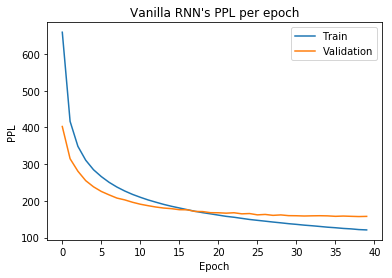
\includegraphics[scale=0.8]{VRNN_LC_EPOCH.png}
	\caption{Vanilla RNN's PPL per epoch}
	\label{fig:fig1}
\end{figure}

\begin{figure}[H]
	\centering
	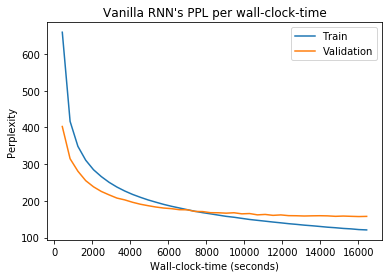
\includegraphics[scale=0.8]{VRNN_LC_TIME.png}
	\caption{Vanilla RNN's PPL per wall-clock-time}
	\label{fig:fig2}
\end{figure}

\begin{figure}[H]
	\centering
	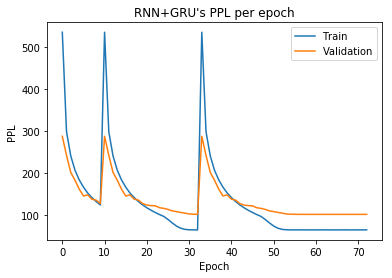
\includegraphics[scale=0.8]{GRU_LC_EPOCH.png}
	\caption{RNN with GRU PPL per epoch}
	\label{fig:fig3}
\end{figure}

\begin{figure}[H]
	\centering
	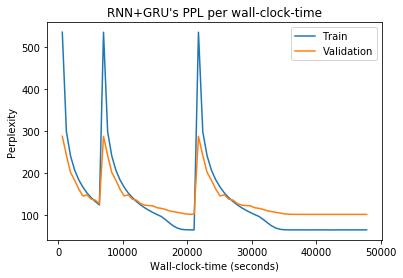
\includegraphics[scale=0.8]{GRU_LC_TIME.png}
	\caption{RNN with GRU PPL per wall-clock-time}
	\label{fig:fig4}
\end{figure}


\subsection{Exploration of optimizers}
In this section we will explore different optimizers for each of the previous models. Each model is run with two different optimizers with the hyperparameters as given in the assignment. 

I\textcolor{red}{nclude the following tables:
	1. For each experiment in 1-3, plot learning curves (train and validation) of PPL over both
	epochs and wall-clock-time.}

\begin{itemize}
	\item[1)] \textbf{Results for Vanilla RNN:}
	The hyperparameters used for experiments 2 and 3 are given in the Table~\ref{table:3}.\\
	\begin{table}[H]
		\centering
		\begin{tabular}{||c c c c||} 
			\hline
			\textbf{Hyperparameters} & \textbf{Experiment 1} &\textbf{Experiment 2} & \textbf{Experiment 3}\\[0.5ex] 
			\hline
			Optimizer & ADAM & SGD & SGD\_LR\_SCHEDULE \\
			Learning rate & 0.0001 & 0.0001 & 1  \\
			Batch size &20 & 20 &20 \\
			Sequence length &35 & 35 & 35\\
			Hidden size & 1500 & 1500 & 512 \\
			Number of layers & 2 & 2 & 2 \\
			Dropout probability & 0.35 & 0.35 &0.35 \\[1ex]
			\hline
		\end{tabular}
		\caption{Vanilla RNN additionnal experiments' hyperparameters}
		\label{table:3}
	\end{table}
	%
	The results of these experiments are shown in  Table~\ref{table:3.1}. We notice that SGD performed worst and could not converge within 40 epochs, whereas ADAM performs best for the same number of epochs and the same hyperparameters. Additionnaly, the SGD\_LR\_SCHEDULE works better than SGD for a bigger learning rate and lower model capacity. In terms of training time, experiment 1 was the slowest, experiment 3 was the fastest while experiment 2 showed an average performance. 
	Given the above setting with the hyperparameters as shown in Table~\ref{table:3}, we conclude that the first experiment (ADAM) is best in terms of performance on the validation set. 
	\begin{table}[H]
		\centering
		\begin{tabular}{||c c c c||} 
			\hline
			\textbf{Result} & \textbf{Experiment 1} & \textbf{Experiment 2}& \textbf{Experiment 3} \\[0.5ex] 
			\hline
			Training PPL & 120.97 & 3008.63 & 229.56 \\
			Validation PPL & 157.82 & 2220.49 & 195.67  \\
			Average time processing per epoch (s) & 411 & 384 & 185 \\[1ex]
			\hline
		\end{tabular}
		\caption{Vanilla RNN results experiments}
		\label{table:3.1}
	\end{table}
	%
	\item[2)] \textbf{Results for GRU:}
	In the experiments 2 and 3, for GRU, we used the parameters given in Table~\ref{table:4}.\\
	%
	\begin{table}[H]
		\centering
		\begin{tabular}{||c c c c||} 
			\hline
			\textbf{Hyperparameters} &\textbf{Experiment 1} & \textbf{Experiment 2} & \textbf{Experiment 3}\\[0.5ex] 
			\hline
			Optimizer & SGD\_LR\_SCHEDULE & SGD & ADAM \\
			Learning rate & 10 & 10 & 0.0001   \\
			Batch size & 20 & 20 &20 \\
			Sequence length & 35 & 35 & 35\\
			Hidden size & 1500 & 1500 & 1500 \\
			Number of layers & 2 & 2 & 2 \\
			Dropout probability & 0.35 & 0.35 &0.35 \\[1ex]
			\hline
		\end{tabular}
		\caption{RNN with GRU additionnal experiments' hyperparameters}
		\label{table:4}
	\end{table}
	%
	The results are shown in Table~\ref{table:4.1}. We notice that SGD\_LR\_SCHEDULE performed best on the validation set, which indicates that it might also generalize well.  With a larger learning rate, SGD performed better than on the Vanilla RNN. ADAM's performance on the training set was best, but its variance was greater than SGD\_LR\_SCHEDULE, which may indicate that the model starts to overfit.
	\begin{table}[H]
		\centering
		\begin{tabular}{||c c c c||} 
			\hline
			\textbf{Result} & \textbf{Experiment 1} & \textbf{Experiment 2}& \textbf{Experiment 3} \\[0.5ex] 
			\hline
			Training PPL & 65.85& 50.33& 59.98 \\
			Validation PPL & 102.63 & 121.36 & 113.71  \\
			Average time processing per epoch (s) & 668 & 648 & 675 \\[1ex]
			\hline
		\end{tabular}
		\caption{First experiment results}
		\label{table:4.1}
	\end{table}
	%
		\item[3)] \textbf{Results for Transformer:}
		The following parameters were used:
		%
		\begin{table}[H]
			\centering
			\begin{tabular}{||c c c c||} 
				\hline
				\textbf{Hyperparameters} &\textbf{Experiment 1} & \textbf{Experiment 2} & \textbf{Experiment 3}\\[0.5ex] 
				\hline
				Optimizer & SGD\_LR\_SCHEDULE & SGD & ADAM\\
				Learning rate & 20 & 20 & 0.001  \\
				Batch size & 128 & 128 & 128 \\
				Sequence length & 35 & 35 & 35\\
				Hidden size & 512 & 512 & 512 \\
				Number of layers & 6 & 6 & 2 \\
				Dropout probability & 0.9 & 0.9 &0.9 \\[1ex]
				\hline
			\end{tabular}
			\caption{The hyperparameters for additional Transformer experiments}
			\label{table:5}
		\end{table}
The following are the results for the transformer:
\begin{table}[H]
	\centering
	\begin{tabular}{||c c c c||} 
		\hline
		\textbf{Result} & \textbf{Experiment 1} & \textbf{Experiment 2}& \textbf{Experiment 3} \\[0.5ex] 
		\hline
		Training PPL & ??? & ??? & ???  \\
		Validation PPL & ???  & ???  & ???  \\
		Average time processing per epoch (s) & ???  & ???  & ???  \\[1ex]
		\hline
	\end{tabular}
	\caption{First experiment results}
	\label{table:5.1}
\end{table}
\end{itemize}
%
In conclusion, assuming that the comparison here was made with a set of hyperparameters that give a fair baseline for all the models, we can say that there is no universal best optimizer regardeless of the model architecture. In fact, each model architecture works better with a suited optimizer. Howerver, we notice that ADAM is a very powerfull optimizer that can make the model converge very quickly. However, if not well-tuned it could make the model overfit the training data. \\

%For the next experiment we will use the best optimizer so far. In order to improve its performance we will do a hyperparameter tuning.



\subsection{Exploration of hyperparmeters}

Figures and Tables:\\
Each table and gure should have an explanatory caption. 
For tables, this goes above, for figures it goes below. 
Tables should have appropriate column and/or row headers.
Figures should have labelled axes and a legend. 

\textcolor{red}{Include the following tables:
1. For each experiment in 1-3, plot learning curves (train and validation) of PPL over both
epochs and wall-clock-time.}

\textcolor{red}{2. Make a table of results summarizing the train and validation performace for each experiment,
	indicating the architecture and optimizer. Sort by architecture, then optimizer, and number
	the experiments to refer to them easily later. Bold the best result for each architecture.}

\textcolor{red}{3. List all of the hyperparameters for each experiment in your report (e.g. specify the command
you run in the terminal to launch the job, including the command line arguments).}

4. Make 2 plots for each optimizer; one which has all of the validation curves for that optimizer
over epochs and one over wall-clock-time.
5. Make 2 plots for each arcitecture; one which has all of the validation curves for that architecture
over epochs and one over wall-clock-time.
\subsection{Discussion}
